% !TeX root = ../main.tex
% Add the above to each chapter to make compiling the PDF easier in some editors.
\chapter{Methodology}\label{chapter:method}
We aim to solve two problems: First the raw dataset being available centrally itself and second the risk of inference attacks. Most research is based on datasets that span only over a few days or weeks. When collecting location data over months, the chance of successful inference attack increases in all cases with more data available.

In order to address the problem and test our hypothesis, we developed a framework in which we collect and locally aggregate location data on end user devices (smartphones). The raw data will stay on each device and will only be used to serve aggregation requests from a central server. The aggregation requests have to be defined upfront. An example is the determination of the average steps per day by each user. An incoming aggregation request might look like
\begin{verbatim}
{
	"n" : 3
	"value": 2000
}
\end{verbatim}
And the data contained in the outgoing response after processing the request might look like
\begin{verbatim}
{
	"n" : 4
	"value": 2500
}
\end{verbatim}
 In order to protect the user's privacy and shield the raw data from the server, it would be necessary to pass the request P2P from one device to another until the last device finally publishes the result to the server. P2P on mobile phones though is hardly possible. Nevertheless, we found a way to oslve this problem: On installation, a public-private key-pair is generated and every installed application registers at the server with this public key. The corresponding private key is stored locally. When one end user device needs to send the processed aggregation request to the next phone, it encrypts the data using that phones public key in the standard hybrid encryption\footnote{In hybrid encryption as used in SSL, the message itself is encrypted with a synchronous key while this key itself is encrypted using the public key} approach leveraging the benefits of synchronous keys. This way the next phone will be able to decrypt the request and process the data while the server is unable to read the data until the aggregation request is finally send in plain text for publishing to the server. This process is depicted in figure XX.

 The aggregated results are available only to our research team in order to protect the research participants privacy in case there is a privacy risk we have not thought of but the setting allows for them being available to the public. The aggregation requsts themselves are controlled by our research team and inserted on a daily basis.

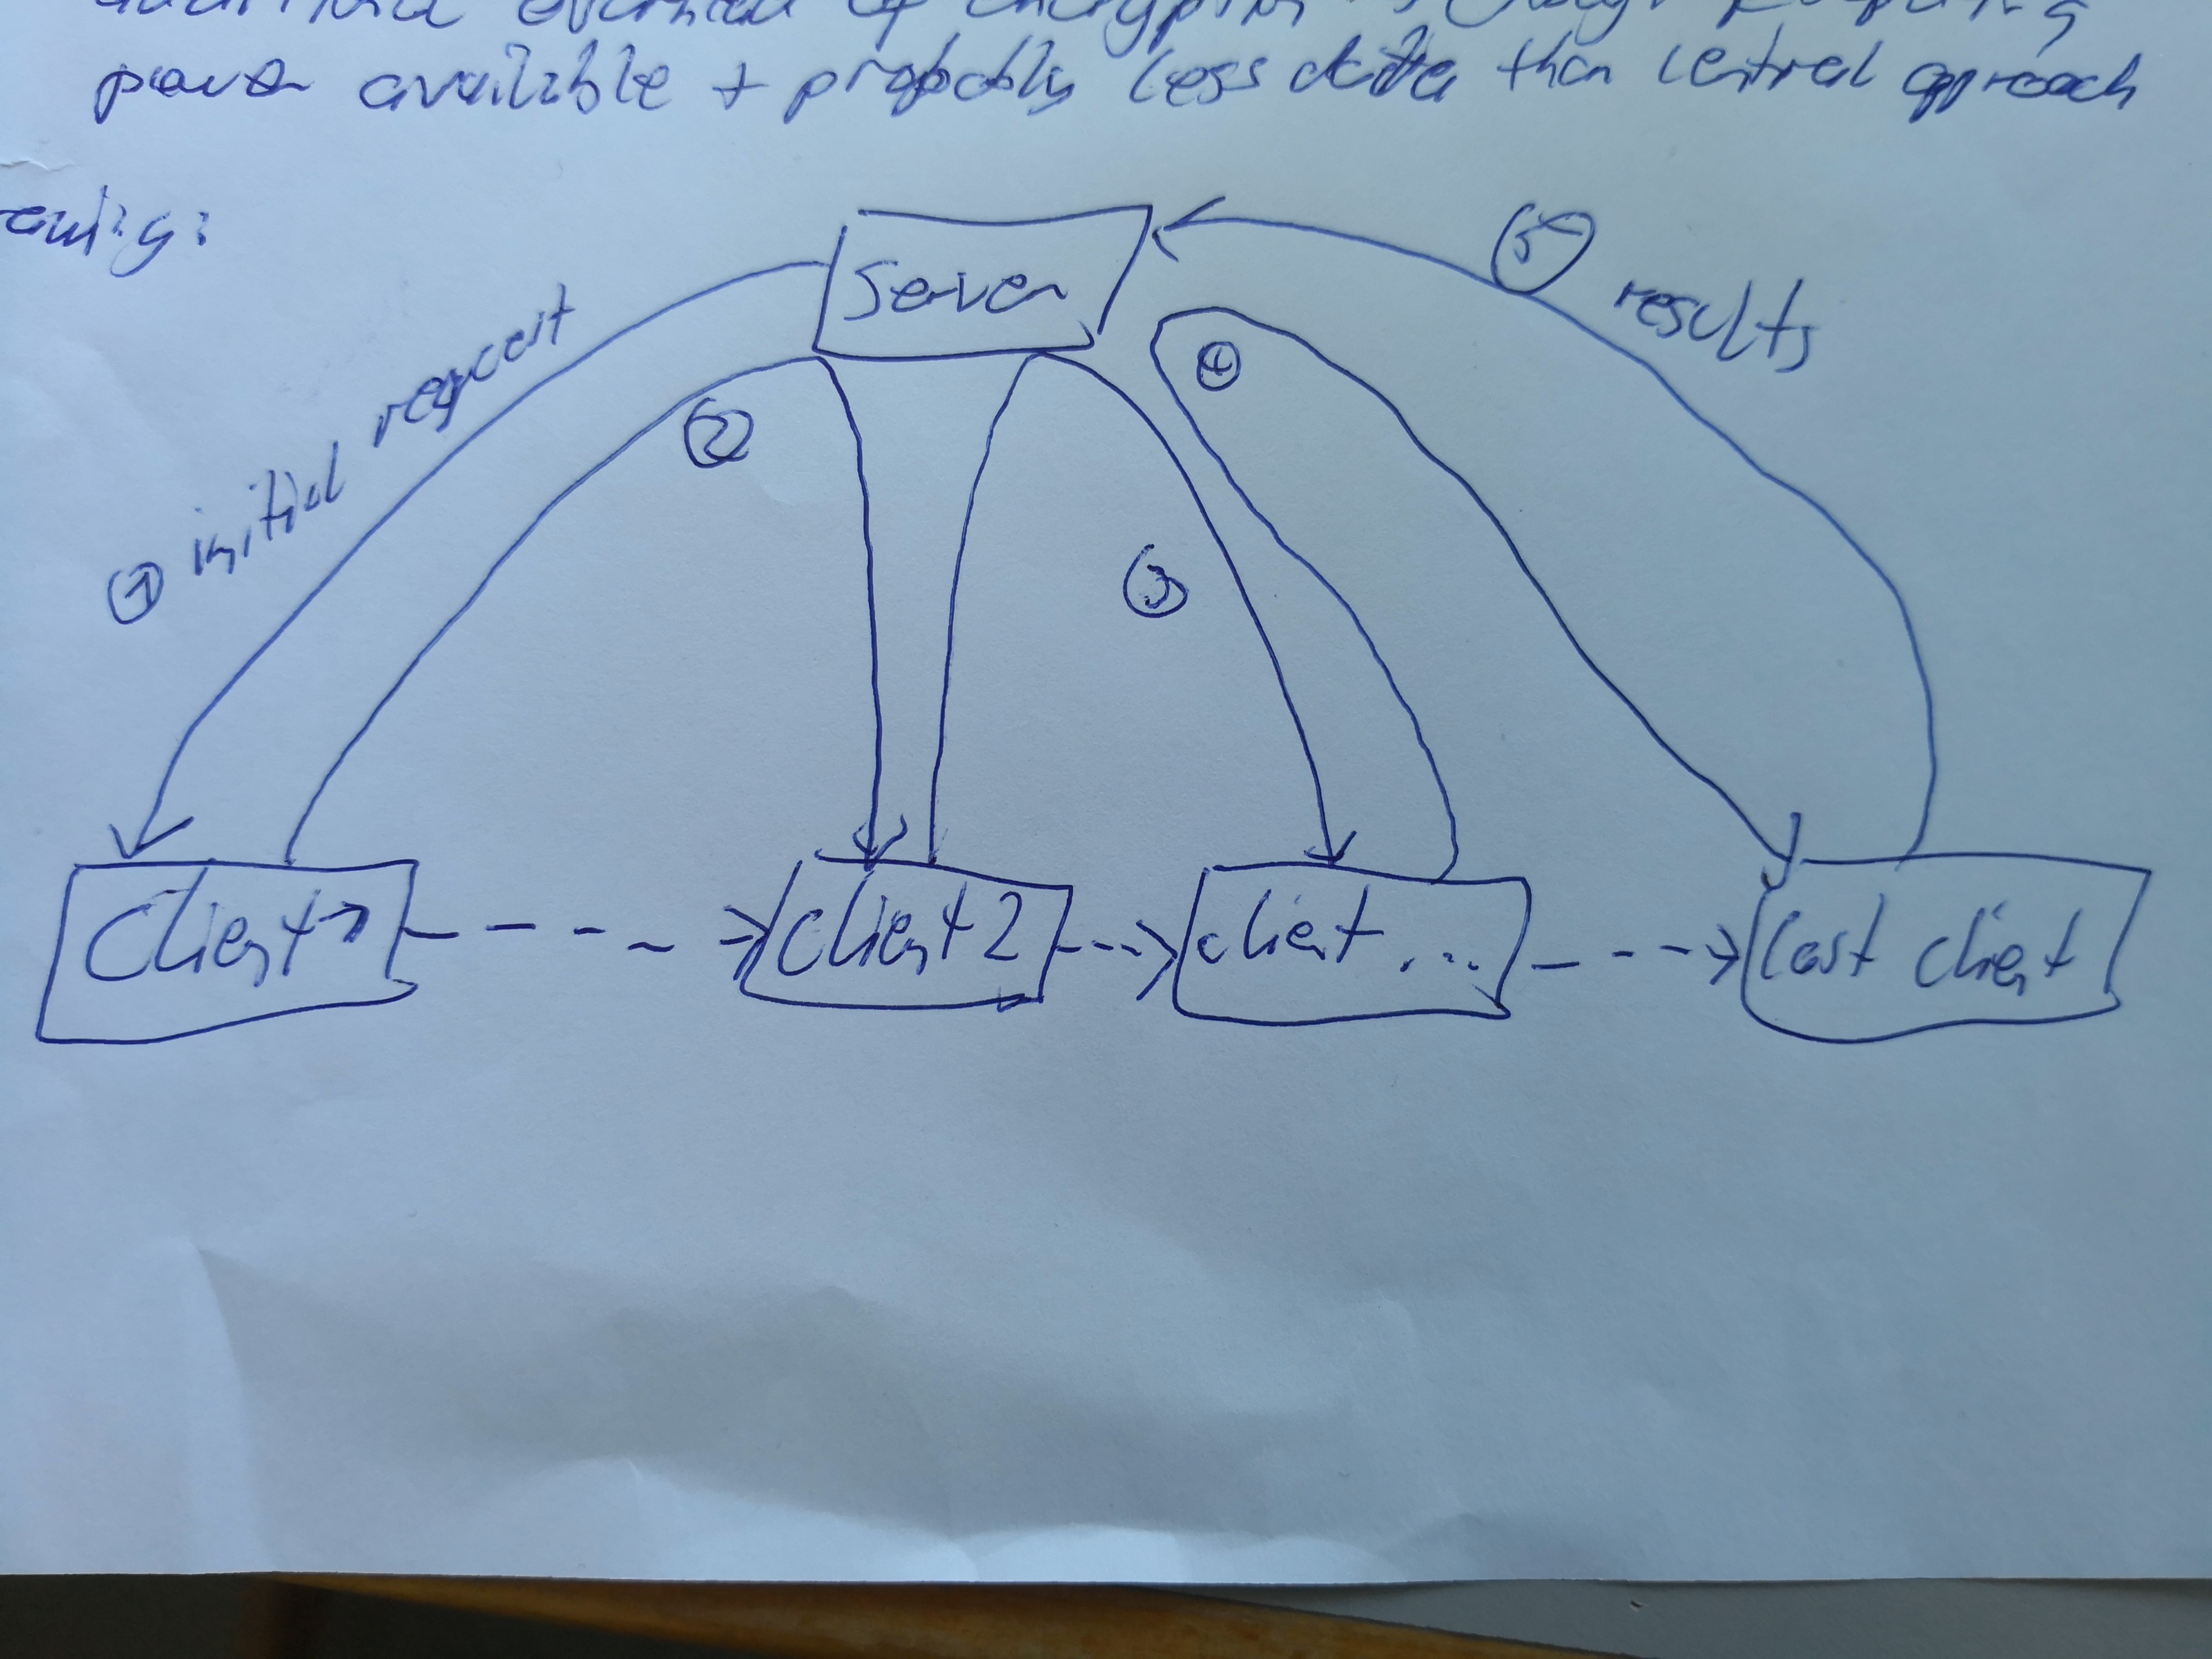
\includegraphics[width=\textwidth]{data/concept.jpg}

